
\begin{figure}[H]
\caption{Lote de tareas ejecutando con Round Robin con quantum 2}
\label{fig:ej5q2}
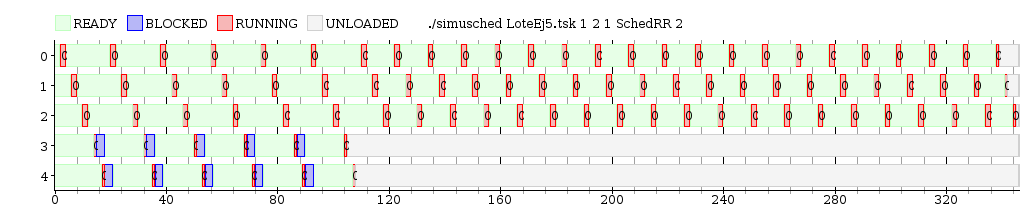
\includegraphics[width=1\textwidth]{imgs/ej5-q2.png}
\end{figure}

\begin{figure}[H]
\caption{Lote de tareas ejecutando con Round Robin con quantum 10}
\label{fig:ej5q10}
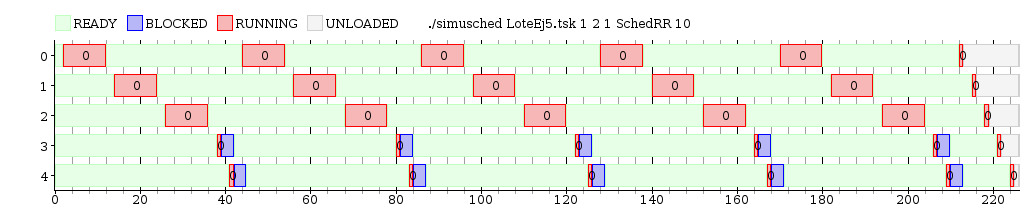
\includegraphics[width=1\textwidth]{imgs/ej5-q10.png}
\end{figure}

\begin{figure}[H]
\caption{Lote de tareas ejecutando con Round Robin con quantum 50}
\label{fig:ej5q50}
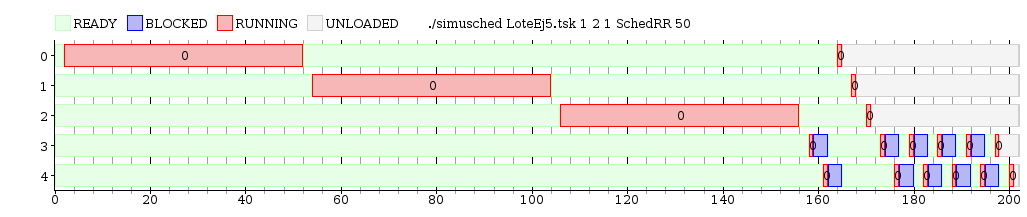
\includegraphics[width=1\textwidth]{imgs/ej5-q50.png}
\end{figure}

\begin{center}
  \begin{tabular}{ c c}
Tarea 0
\begin{tabular}{| l | c | c | c |}
\hline  
\textbf{Quantum} & \textbf{2} & \textbf{10} & \textbf{50} \\ \hline
Latencia & 2 & 2 & 2 \\ \hline
Waiting Time & 288 & 162 & 114 \\ \hline
Tiempo Total & 339 & 213 & 165 \\ \hline
\end{tabular}&


Tarea 1
\begin{tabular}{| l | c | c | c |}
\hline  
\textbf{Quantum} & \textbf{2} & \textbf{10} & \textbf{50} \\ \hline
Latencia & 6 & 14 & 54 \\ \hline
Waiting Time & 291 & 165 & 117 \\ \hline
Tiempo Total & 342 & 216 & 168 \\ \hline
\end{tabular} \\[3em]

Tarea 2
\begin{tabular}{| l | c | c | c |}
\hline  
\textbf{Quantum} & \textbf{2} & \textbf{10} & \textbf{50} \\ \hline
Latencia & 10 & 26 & 106 \\ \hline
Waiting Time & 294 & 168 & 120 \\ \hline
Tiempo Total & 345 & 219 & 171 \\ \hline
\end{tabular} &



Tarea 3 
\begin{tabular}{| l | c | c | c |}
\hline  
\textbf{Quantum} & \textbf{2} & \textbf{10} & \textbf{50} \\ \hline
Latencia & 14 & 38 & 158 \\ \hline
Waiting Time & 84 & 201 & 177 \\ \hline
Tiempo Total & 105 & 222 & 198 \\ \hline
\end{tabular} \\[3em]

Tarea 4
\begin{tabular}{| l | c | c | c |}
\hline  
\textbf{Quantum} & \textbf{2} & \textbf{10} & \textbf{50} \\ \hline
Latencia & 17 & 41 & 161 \\ \hline
Waiting Time & 87 & 204 & 180 \\ \hline
Tiempo Total & 108 & 225 & 201 \\ \hline
\end{tabular} & \\

\end{tabular}

\end{center}

\hspace{4em}

\begin{figure}[H]
\caption{Valores Promedio entre las tareas}
\label{fig:ej5-tabla}
\begin{center}
\begin{tabular}{| l | c | c | c |}
\hline  
\textbf{Quantum} & \textbf{2} & \textbf{10} & \textbf{50} \\ \hline
Latencia & 9.8 & 24.2 & 96.2 \\ \hline
Waiting Time & 208.8 & 180 & 141.6 \\ \hline
Tiempo Total & 247.8 & 219 & 180.6 \\ \hline
\end{tabular}
\end{center}
\end{figure}

Conclusiones a partir de los gráficos (figuras \ref{fig:ej5q2}, \ref{fig:ej5q10} y \ref{fig:ej5q50}, además de la tabla de la figura \ref{fig:ej5-tabla}): 

\begin{itemize}

\item Con respecto a la \textbf{latencia}, es menor en el caso con el scheduler con quantum de 2 ciclos. Esto se debe a que el primer desalojo se hace más rápido ya que el tiempo asignado por quantum es menor que en los demás. Como se ve en la tabla de los promedios, el valor de la latencia aumenta cuanto mayor es el valor del quantum.
\item Con respecto al \textbf{waiting time}, ocurre lo contrario, es menor con el scheduler de quantum 50. Esto se debe a que cuanto menor es el quantum, más cambios de contexto se realiza durante la ejecución de las tareas, y esto agrega tiempo de espera ya que cada cambio de contexto tarda 2 ciclos en realizarse.
\item Por último, el \textbf{tiempo total}, al igual que en el anterior, es menor en último caso, con quantum de 50 ciclos. De la misma manera, al aumentar el quantum y reducir los cambios de contexto, y por ende los costos de cada cambio de contexto, el tiempo total se reduce.
\end{itemize}



